\chapter{Validazione}
\label{chap:validazione}

\section{Test automatici}
\label{sec:test-automatici}

Il modulo è stato validato tramite una suite di test scritta con
Kotest~\footnote{Kotest: \url{https://kotest.io/}.},
che conta 209 test unitari.
Le classi di test sono disposte seguendo la struttura dei package del codice,
così che a ogni componente corrisponda il test che lo verifica, e sono
eseguite dalla pipeline di integrazione continua di Alchemist su Linux,
macOS e Windows, assieme agli strumenti di analisi statica adottati
dal progetto.

Il valore atteso dai test non è mai ottenuto ripetendo lo stesso calcolo
svolto dal codice da verificare. I valori attesi sono invece calcolati
a mano su casi di piccole dimensioni, prodotti da strumenti esterni,
oppure derivati da proprietà che il risultato corretto deve soddisfare.
Ad esempio, i digest MD5 attesi sono calcolati con \texttt{md5sum}, e fra
i contenuti usati ne compare uno il cui digest comincia con due cifre nulle,
così da verificare la normalizzazione descritta nella \Cref{subsec:integrita-impl}.

I file NetCDF usati dai test non sono archiviati nel repository, ma generati
a ogni esecuzione con valori noti. In questo modo è possibile controllare
esattamente le proprietà che la lettura deve normalizzare (\Cref{subsec:normalizzazione-impl}):
lo stesso contenuto viene scritto con ordini delle dimensioni e direzioni degli assi diversi,
e si verifica che la serie letta sia in ogni caso la stessa.
Il formato GRIB, che la libreria sa leggere ma non sa scrivere, è coperto nei test
da un file reale estratto dai data store, incluso fra le risorse di test.

Di seguito, nel \Cref{lst:test-raster}, è mostrato un esempio di questi test:
la verifica delle realizzazioni di \texttt{RasterGrid}.

\lstinputlisting[
    language=Kotlin,
    label={lst:test-raster},
    caption={[Verifica delle implementazioni di RasterGrid.]Verifica delle implementazioni di \texttt{RasterGrid}.}
]{listings/validazione/TestRasterGrid.kt}

Il \Cref{lst:test-provider} mostra la simulazione completa della sequenza di recupero dati dai data store tramite \texttt{CopernicusDataStoreProvider}.
Il test mostra lo scambio sulla base di risposte reali catturate dal servizio \ac{CDS} a fronte di una richiesta effettiva.

\lstinputlisting[
    language=Kotlin,
    label={lst:test-provider},
    caption={[Simulazione della sequenza di recupero da un data store.]Simulazione della sequenza di recupero dal data store CDS.}
]{listings/validazione/TestCopernicusDataStoreProvider.kt}

Il requisito \req{NF3}, il quale richiede che i test non dipendano
dalla disponibilità dei data store, è soddisfatto a livelli differenti:

\begin{itemize}
  \item il layer è verificato tramite il costruttore che riceve una serie già
  disponibile, costruita dinamicamente nei test, e usando un environment fittizio
  il cui tempo di simulazione è fissato dal test stesso;
  \item il gestore della cache è verificato tramite una fonte fittizia, che
  conta le proprie invocazioni e può essere istruita a fallire, a non produrre
  file o a fallire dopo averne prodotti alcuni;
  \item il client dei data store dialoga con un server HTTP locale,
  realizzato con quello incluso nel JDK (\texttt{com.sun.net.httpserver}), che
  riproduce i corpi di risposta catturati da richieste reali ai tre data store.
  Prima di essere serviti, gli indirizzi dei data store reali vengono
  sostituiti con quello del server locale, in modo che non avvenga mai
  una richiesta reale verso l'API di ECMWF.
\end{itemize}

\section{Verifiche al di fuori dei test}
\label{sec:verifiche-manuali}

La compatibilità con il caricamento (\req{F11}) è la parte del modulo più
condizionata da vincoli esterni (\Cref{subsec:costruttori-impl}), e non è
verificata dai test automatici, i quali costruiscono il layer direttamente.
La verifica è avvenuta in due modi distinti. Il primo è tramite il bytecode:
l'ispezione con \texttt{javap} della classe compilata conferma che 
\texttt{@JvmOverloads} genera tutte le varianti dei costruttori eliminando un argomento
opzionale per volta, partendo dall'ultimo di questi.
Il \Cref{lst:javap} riporta un estratto dell'output di \texttt{javap} che comprende le
varianti del secondo costruttore di \texttt{DoubleCopernicusLayer}.

\lstinputlisting[
    language={},
    keywordstyle={},
    stringstyle={},
    commentstyle={},
    label={lst:javap},
    caption={[Estratto dell'output di javap]Estratto dell'output di \texttt{javap}; i nomi dei package sono omessi.}
]{listings/validazione/javap.txt}

La seconda modalità è il caricamento effettivo: la configurazione della 
simulazione dimostrativa (\Cref{sec:caso-di-studio}) e alcune sue varianti, che omettono
suffissi diversi dagli argomenti facoltativi o selezionano strategie
diverse, sono state caricate ed eseguite con successo.

In particolare, il client è stato esercitato con successo su tutti e tre i data store
reali, con richieste a diversi dataset su ciascuno di essi.
I corpi di risposta, usati come dati di verifica successivamente nei test,
sono stati catturati proprio da queste esecuzioni, e i file scaricati sono stati letti
dal modulo senza errori. È proprio in questa fase che sono stati scoperti
molti degli scostamenti dal protocollo discussi nel \Cref{chap:implementazione}.

\section{Simulazione dimostrativa}
\label{sec:caso-di-studio}

Questa sezione mostra l'intera catena del modulo all'opera su dati reali:
la richiesta verso il data store, la conservazione dei dati nella cache locale,
la loro lettura da parte dei nodi durante la simulazione e il riuso in
un'esecuzione successiva. La simulazione è a scopo solamente dimostrativo
rispetto al modulo: il comportamento dei nodi è volutamente elementare
e non intende modellare un atteggiamento verosimile.
Ciò che si vuole verificare non è cosa facciano i nodi, ma che reagiscano ai
valori esposti dal layer, nel punto e nell'instante corretti.

\subsection{Scenario e dati}

Lo scenario riprende l'alluvione che tra il 2 e il 17 maggio 2023 ha colpito la Romagna.
Durante l'evento il fiume Savio, come altri corsi d'acqua del territorio,
è straripato. I dati dell'alluvione provengono dal dataset \texttt{efas-historical}
di \ac{EWDS} nella versione 5.0 del sistema~\cite{JRC134686}, il quale espone i dati
tramite una griglia latitudine-longitudine regolare, a differenza delle versioni precedenti
che espongono in proiezione \ac{LAEA}. Questa versione del modello presenta
una risoluzione di un minuto d'arco in latitudine e longitudine, una misura angolare,
corrispondente a circa 1.9 km in latitudine e 1.3 km in longitudine sulle coordinate
di Cesena.
La variabile richiesta è la portata fluviale media nelle sei ore precedenti,
ovvero la quantità media di acqua che attraversa una determinata sezione di
un fiume nell'unità di tempo (misurata in $\frac{m^{3}}{s}$),
fornita a intervalli di sei ore. Il \Cref{lst:richiesta-efas} riporta i parametri
della richiesta al dataset.

\lstinputlisting[
    language=json,
    label={lst:richiesta-efas},
    caption={Richiesta al dataset \texttt{efas-historical} per la simulazione dimostrativa.}
]{listings/exemplar/alluvione_cesena.json}

In questo dataset i campi \texttt{hmonth} e \texttt{hday} indicano i mesi e
giorni selezionati. I dati richiesti osservano la portata fluviale dall'inizio di aprile
fino alla fine di giugno 2023. Vengono richieste tutte le griglie disponibili nell'arco
della giornata (una ogni sei ore). Il parametro \texttt{model\_levels} viene
specificato anche se non ha un uso effettivo: altre variabili dello stesso dataset
possono essere campionate a più livelli, la portata idrica invece solo sulla superficie.
Il parametro \texttt{area} delimita la zona di studio; in questo caso viene selezionato
un rettangolo che include l'intera città di Cesena.

\subsection{Configurazione}

Il \Cref{lst:yaml-dimostrativa} riporta la parte della configurazione che
riguarda il modulo: la dichiarazione del layer nella modalità da data store
(\Cref{subsec:costruttori-impl}) e la condizione di terminazione.

\lstinputlisting[
    float,
    language=YAML,
    label={lst:yaml-dimostrativa},
    caption={[Configurazione del layer]Dichiarazione del layer e condizione di terminazione nella simulazione dimostrativa.}
]{listings/exemplar/emilia-romagna-2023-evacuazione.yaml}

Gli ultimi due parametri del layer fissano la corrispondenza temporale:
un'unità di tempo simulato
corrisponde a un'ora reale, e il tempo zero al 25 aprile 2023, ore 00:00 UTC. Il
valore di \texttt{timeScale} coincide con quello predefinito, ma va indicato
perché il sistema di caricamento, per assegnare per nome un parametro opzionale, richiede anche
tutti quelli che lo precedono. Con questa
scala e origine, facendo terminare la simulazione dopo 1584 unità di
tempo simulato, si chiude la riproduzione dell'evento con i dati
del 30 giugno 2023, ore 00:00 UTC.

L'ambiente è un \texttt{OSMEnvironment} (Sezione~\ref{subsec:alchemist-osm})
costruito su un estratto OpenStreetMap di Cesena.
Ogni nodo esegue un programma che, una volta per unità di tempo simulato,
legge il layer nella propria posizione. Il comportamento si riduce a una soglia
della portata fluviale: una volta superata quest'ultima, il nodo entra in stato di allarme
e viene portato a spostarsi verso punti di uscita prestabiliti utilizzando il grafo
stradale.

L'intervallo di valori assunti dai dati è stato identificato analizzando il dataset
tramite Panoply~\footnote{Panoply, visualizzatore di dati geospaziali della NASA: \url{https://www.giss.nasa.gov/tools/panoply/}.}.
La portata fluviale descritta dai dati raccolti va da un minimo di 0 a un massimo di 4.6 $\frac{m^{3}}{s}$.
Si è scelto di usare 3.5 $\frac{m^{3}}{s}$ come soglia di allarme per i nodi.

\subsection{Esecuzione}

Alla prima esecuzione la richiesta non è in cache. Il \Cref{lst:log-cache-miss}
riporta i messaggi con cui il modulo segnala l'acquisizione: la prima e l'ultima riga
provengono dal gestore della cache, le altre dal client dei data store, che segue il flusso
asincrono di sottomissione, attesa e scaricamento descritto nella \Cref{subsec:ciclo-richiesta-impl}.

\lstinputlisting[
    language={},
    keywordstyle={},
    stringstyle={},
    commentstyle={},
    label={lst:log-cache-miss},
    caption={[Log della prima esecuzione.]Messaggi del modulo alla prima esecuzione, con la richiesta assente dalla cache. Prefissi del logger omessi, percorsi abbreviati.}
]{listings/validazione/cache_miss.txt}

Una volta recuperati con successo i dati, la simulazione viene avviata.
La \Cref{fig:caso-studio} mostra l'esecuzione in istanti successivi.
Il campo colorato di blu è la portata esposta dal layer, resa con un effetto
grafico realizzato per questa simulazione. Una zona senza colore non indica
necessariamente una portata fluviale nulla: l'effetto non colora zone
con una portata inferiore a 2 $\frac{m^{3}}{s}$.

\begin{figure}[H]
  \centering
  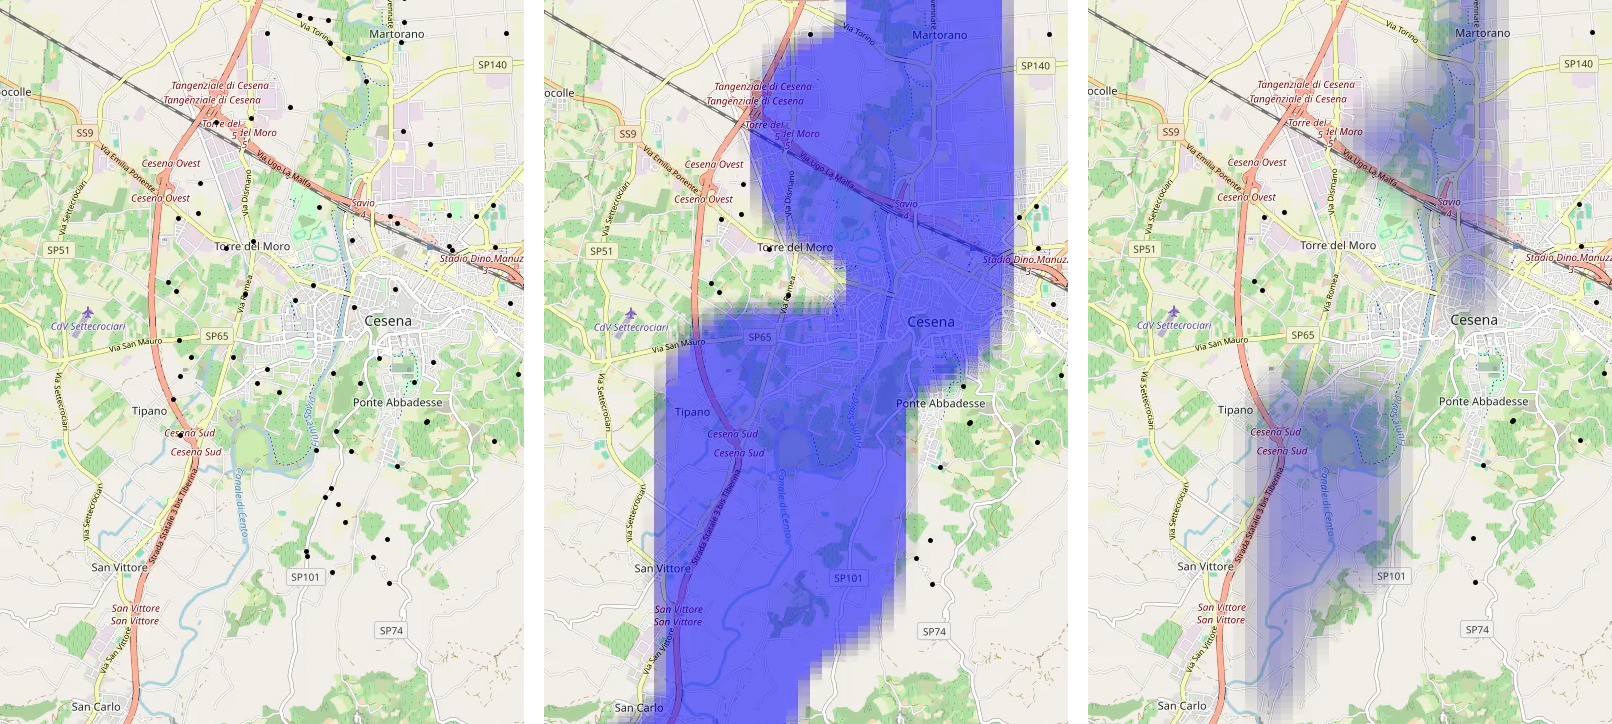
\includegraphics[width=\linewidth]{figures/validazione/alluvione.png}
  \caption[La simulazione dimostrativa in istanti successivi]{La simulazione in
  tre istanti successivi. Da sinistra: prima degli eventi,
  durante l'esondazione del fiume Savio, la riduzione della portata.}
  \label{fig:caso-studio}
\end{figure}

Nelle immagini, in ordine da sinistra verso destra:

\begin{enumerate}
  \item 25 aprile 2023, 00:00 UTC (tempo di simulazione 0): la portata fluviale
  del fiume Savio rientra nella norma;
  \item 16 maggio 2023, 15:00 UTC (tempo di simulazione 519): il fiume Savio straripa.
  I nodi che rilevano nella propria posizione un valore oltre la soglia di allerta
  si spostano fuori dalla zona;
  \item 21 maggio 2023, 04:00 UTC (tempo di simulazione 580): la portata fluviale
  si riduce. I nodi che sono stati allertati rimangono fuori dalla zona.
\end{enumerate}

Riavviando la simulazione con la stessa configurazione, il gestore della cache
trova la voce e il layer viene costruito senza alcuna richiesta di rete
(\Cref{lst:log-cache-hit}), a verifica di \req{F9} e \req{F10}.

\lstinputlisting[
    language={},
    keywordstyle={},
    stringstyle={},
    commentstyle={},
    label={lst:log-cache-hit},
    caption={[Log della seconda esecuzione.]{Messaggio del modulo alla seconda esecuzione con la stessa configurazione. Prefisso del logger omesso.}}
]{listings/validazione/cache_hit.txt}

La chiave della voce è derivata dall'endpoint, dal dataset e dal contenuto della
richiesta. I parametri che non ne fanno parte, come l'origine temporale o la
strategia di interpolazione, possono quindi cambiare fra un'esecuzione e l'altra
senza provocare un nuovo scaricamento.

L'esecuzione è stata ripetuta con successo anche eliminando il file \texttt{.cdsapirc},
il quale contiene la chiave ECMWF, a conferma che esso viene letto solo quando
una richiesta di rete si rende necessaria.